\documentclass[conference]{IEEEtran}
\IEEEoverridecommandlockouts
% The preceding line is only needed to identify funding in the first footnote. If that is unneeded, please comment it out.
\usepackage{cite}
\usepackage{amsmath,amssymb,amsfonts}
\usepackage{algorithmic}
\usepackage{graphicx}
\usepackage{textcomp}
\usepackage{xcolor}
%\usepackage[T1]{fontenc}
%\usepackage[polish]{babel}
\usepackage[utf8]{inputenc}
\def\BibTeX{{\rm B\kern-.05em{\sc i\kern-.025em b}\kern-.08em
    T\kern-.1667em\lower.7ex\hbox{E}\kern-.125emX}}
\begin{document}

\title{Distributed Oscilloscope over White Rabbit Network\\
}

\author{\IEEEauthorblockN{ Miłosz Malczak, Grzegorz Kasprowicz}
\IEEEauthorblockA{\textit{The Faculty of Electronics  and Information Technology} \\
\textit{Warsaw University of Technology}\\
Poland }

\and
\IEEEauthorblockN{Dimitrios Lampridis}
\IEEEauthorblockA{\textit{Beams Department, Controls Group}\\
\textit{CERN}\\
Geneva, Switzerland }
}

\maketitle

\begin{abstract}
The Distributed Oscilloscope is a system allowing monitoring of signals located over large distances. It is built on top of the White Rabbit Trigger Distribution, which uses the White Rabbit Network to provide subnanosecond synchronization. The goal of the Distributed Oscilloscope is to overcome the problems of existing devices: lack of precision, compatibility and scalability.  


\end{abstract}

\begin{IEEEkeywords}
White Rabbit, oscilloscope, trigger
\end{IEEEkeywords}

\section{Introduction}

% description of the problem 
Large-scale scientific installations like particle accelerator facilities, metrological laboratories, radar arrays, power grids and many others require monitoring of signals in devices that could be located kilometres away from each other. Currently, such measurement systems exist, but have some of the following disadvantages: they are custom-made, not scalable, not precise enough and suffer from the lack of compatibility.

% solution
The Distributed Oscilloscope overcomes all of these problems. It uses White Rabbit Trigger Distribution (WRTD), which allows sending the triggers in digital form to specified devices. The precision is obtained by the use of the White Rabbit (WR) network. WR is being introduced to the IEEE 1588 Precision Time Protocol (PTP) standard, hence it is well documented. Since WR is becoming a standard, other systems that are built on top of it will be compatible with each other. The Distributed Oscilloscope is written in Python, so its implementation could be easily understood by a non-expert programmer and thanks to its modular structure allows users to modify it according to their needs, as well as to pick some parts of it to introduce in their own system. In order to make it suitable for common use, it is going to be compatible with LAN-based eXtensions for Instrumentation (LXI) and Interchangeable Virtual Environments Foundation (IVI), which are consortiums that standardize access to various types of instrumentation. 

%implementation hidden from the user
The way devices communicate with each other and how the data is synchronized, are hidden from the users. From their perspective, adding the possibility of displaying data from various devices means just adding another trigger source in the standard oscilloscope.

% description of the document
In section II existing solutions are briefly described.
In section III the general architecture of the system is shown.  
In section IV the White Rabbit Trigger Distribution project is presented.
In section V the current progress of the project is presented, as well as the improvements that are going to be introduced in future versions.

\section{Existing solutions}

\subsection{LXI}
LXI standardizes access to various types of instrumentation, its configuration and data acquisition. It also provides optional functionalities for synchronization of devices, based on the IEEE 1588-2002 Precision Time Protocol. The accuracy of clock synchronization in PTP is in the range of 1 microsecond. This is not sufficient for many applications, where the frequency of the clock is in the range of tens or hundreds of MHz. For this reason, to our best knowledge, there are no devices that support the optional synchronization features of LXI.

\subsection{OASIS}
%How it works
The OASIS system is currently used at CERN for monitoring signals in its accelerators and experiments. It uses digitizers to sample the signals. The samples are sent to a server that manages all the connections and sends them to applications which provide a Graphical User Interface (GUI).

%Implementations
In order to be able to display the data as if it came from the same device, all digitizers need to receive a synchronized trigger pulse. To achieve that, coaxial cables are used to distribute the pulses. In order to compensate for different logical latencies and different cable lengths, delay logic is introduced for each signal path\cite{b1}. In practice, users usually display the data from devices located close to each other and they don't need to compensate for the latencies.  The main drawbacks of this approach are the complexity of the infrastructure since all digitizers require a separate coaxial cable and lack of proper synchronization. 

\section{Distributed Oscilloscope}

Distributed Oscilloscope consists of three blocks: ADC, Server and GUI. ADCs are installed in Front End Computers (FEC) --- computers that serve as hosts for the hardware. ADCs exchange triggers over the White Rabbit Network. The rest of the system is communicated over standard Ethernet network. The architecture of the system is shown in Fig.\ref{dist_osc} 

\begin{figure}
\centerline{\includegraphics{images/distributed_oscilloscope.png}}
\caption{Distributed Oscilloscope scheme.}
\label{dist_osc}
\end{figure}


\subsection{Analogue to Digital Converter}
%description of the access to ADC
Access to the ADC is provided by a C library, for which a python wrapper was written.

%how it workd
The FEC notifies the Server about its presence. After establishing the connection, the Server informs the FEC about its IP address and retrieves the current configuration from the ADC. One thread is responsible for configuring the ADC according to the Server's requests. The other thread is responsible for retrieving the acquisition data after the trigger has arrived and sending it to the Server. 

\subsection{Graphical User Interface}
%what it is
%For Dimitris it is bad english and You should find some better name for the GUI
The GUI application allows easy interaction of the user with the system.

%How it works
Just like in the case of the FEC, the GUI notifies the Server about its presence. After that one thread is responsible for interaction with the user. The second thread communicates with the Server. Whenever the user wants to reconfigure an ADC, the GUI sends a request to the server. The value displayed in the GUI is changed only after receiving confirmation from the server that the modification was successful. Whenever the data is received from the server, it is plotted in the GUI. 

\subsection{Server}
%What it is
The Server is the central unit responsible for communication with all devices and user interfaces.

%How it works
It manages all requests and determines if they could be applied, as well as keeps track of the ADCs connected to the users. Whenever the data is received, the Server checks which of the users has requested the data from certain ADC and also if the data from other ADCs has arrived. Then it checks if the triggers are properly aligned. Only after that, it sends the data to the user. The server also has to check if the required change in the configuration of the ADC was successfully applied. 

Users can connect in the slave mode (just to display the data) or in the master mode (with the possibility to configure devices). This is necessary in the distributed system, in order to make sure that the ADC that is being used by one user is not reconfigured by another one, however, the possibility to display the data from the device should not be restricted just to one user. 


\section{White Rabbit Trigger Distribution}
%Whta it is, the main goal
The goal of the WRTD is to deliver timestamps to various devices. Timestamps represent the time of the triggers. When they are recieved they determine when the device should trigger. Just like in the case of OASIS, in order to be able to display the data with the actual phase relationship, compensation for different logical latencies and different cable lengths must be introduced. In the case of the Distributed Oscilloscope, it is not required that every node triggers at exactly the same time, but to be able to define what is the exact delay between the triggers. With this knowledge, appropriate compensation is introduced afterwards. Nevertheless, the timestamps must be delayed, which means adding a constant value to the timestamp, so that the receiving nodes are able to trigger. Without introducing the delay, the received timestamp would represent the instance in the past, consequently would not cause the device to trigger.


\subsection{White Rabbit Network}
%common time refernece
WRTD can work only if all devices share the same time reference. Without it, blocks located far away from each other would have no means to determine when to trigger with respect to other blocks. The common time reference is obtained using the White Rabbit network, which provides a 125 MHz clock, synchronised with subnanosecond precision\cite{b2}.

%transmission delays
The second feature obtained from the WR is the knowledge of transmission delays over the fibre. Knowing these values, as well as the delays of hardware components, the worst case transmission delays between all nodes can be calculated. In order to deal with different delays between the nodes, the White Rabbit Trigger Distribution system allows programming of input and output delays. Since White Rabbit is based on the Ethernet, it allows sending data packets over the network. This feature is used to send the timestamps over WRTD.


\subsection{White Rabbit Trigger Distribution block}

The basic block used in the White Rabbit Trigger Distribution is presented in Fig.\ref{wrtd}.

\begin{figure}
\centerline{\includegraphics{images/wrtd.png}}
\caption{White Rabbit Trigger Distribution block.}
\label{wrtd}
\end{figure}

%description of hardware
The arrows in the figure represent inputs and outputs of the block. Local in and local out are connections for devices located in the same Front End Computer. Any devices that generate or receive timestamps could be connected to them. Typical input devices are Time to Digital Converters (TDC), that convert external pulses into timestamps, or Analog to Digital Converters (ADC) that produce the timestamps when a measured value crosses the predefined threshold voltage. Typical output devices are Fine Delays generators --- devices that produce a pulse based on the received timestamp, or WRTD enabled Analogue to Digital Converters, that trigger at the time specified by the timestamp. Remote in and remote out represent connections with different White Rabbit Trigger Distribution blocks. Both local and remote connections operate only on the timestamps. The only difference is that the local connections are predefined for the use with local devices and other connections are considered remote.

\subsection{WRTD in Distributed Oscilloscope}
There are two methods of triggering the ADCs in such a way that the data received from them could be displayed as if it came from the same device:
\begin{enumerate}
\item 
Programming the time when the ADCs should be triggered. 
\item
Triggering the ADCs based on the timestamp received from the other ADC. 
\end{enumerate}

In the first case, only the timestamp is sent to the device. Whenever the actual time is equal to the timestamp, the device triggers. For this approach the WRTD is not required --- all that is needed is a common notion of time that is assured by the White Rabbit network.

The scheme for the second approach is illustrated in Fig.\ref{trig_prop}. 

\begin{figure}
\centerline{\includegraphics{images/trigger_propagation.png}}
\caption{Trigger propagation scheme.}
\label{trig_prop}
\bigskip
\end{figure}


When one of the ADCs receives the trigger it acquires the data and propagates the timestamp to other ADCs. Since the worst-case propagation delay between all nodes is known, the delay introduced by the WRTD to the timestamp is set. In order to make sure that each received timestamp will represent a moment in the future:\\
\begin{equation}
\Delta t_i >= \delta_i
\end{equation}
$\Delta t_i$ ---  delay introduced by WRTD\\
$\delta_i $ ---  propagation delay of the network \\

The number of postsamples and presamples (samples that are acquired after and before receiving the trigger) is programmed by the user.
ADCs acquire the data constantly and write it to the buffer. Whenever the timestamp is received, the data is read, with the number of presamples and postsamples calculated:\\
\begin{align}
\text{presamples} & = \text{presamples}_\text{required} + \Delta t * f_s , \\
\text{postsamples} & = \text{postsamples}_\text{required} - \Delta t * f_s, 
\end{align} 
$f_s$ - sampling frequency of the ADC. \\
Currently the ADC does not support programming negative value of postsamples, so additional number of data is acquired, but only the required data is sent to the Server.

This way the data obtained from the ADC corresponds to the same instance of time. After the acquisition, data from all ADCs is sent to the Server and then to the GUI. The data is displayed to the user as if it came from the same module.
Whenever the buffer is too short to record the necessary number of data, it returns as many samples as available.

In the more generic case, the system should support TDCs as sources of timestamps as well as communication with the ADCs directly over White Rabbit. That would allow using them without Front End Computers. This approach would require significant changes in the HDL design of supported boards. 


\section{Current progress and future work}
%Current
The basic Distributed Oscilloscope with a possibility of specifying the time of the triggers is already implemented. Currently, the work on including WRTD is in progress. 

%Future
The Distributed Oscilloscope will be made more generic. At the moment it supports only one type of ADC. In the future, it will support different ADCs, as well as TDCs, providing a common interface for different types of devices. Additional functions available in standard oscilloscopes will be implemented, as well as the possibility to display the White Rabbit network topology in the form of a graph.
In order to improve the precision of timestamping, the design of the currently used ADC will be improved, locking its sampling clock to the White Rabbit clock. Support for communication directly over WR will be added at last. 




\begin{thebibliography}{00}
%\bibitem{b2} J. Varela, Timing and synchronization in the LHC Experiments, 6th Workshop on Electronics for LHC Experiments, Kraków, 2000.
\bibitem{b1} K. Sigerud (2017, November 9). OASIS - Open Analogue Signal Information System. Retrieved from \textit{https://be-dep-co.web.cern.ch/content/oasis.}
\bibitem{b2} T. Włostowski, ``Precise time and frequency transfer in a White Rabbit Networks,'' M.S. thesis, Warsaw University of Technology, 2011.
\end{thebibliography}
\end{document}
